\chapter{Object definition and preselection}\label{ch4}


The $t\bar{t}$ pairs, produced in proton-proton collisions at the LHC, decay immediately after their creation and leave a unique signature in the detector, which allows to distinguish the interesting events from the physical background. However, the observed signature in the detector gives only hints about the decay products of the top-quark pair.
In case of the lepton + jets channel, these decay products are electrons, muons, jets and a certain amount of missing transverse energy, corresponding to the neutrino. In order to identify these objects, one has to introduce a definition of the different physical objects, which are required for measurements. Hence, the decay products of the $t\bar{t}$ final states are connected with the quantities measured by the experiment.

All definitions which are used in terms of this analysis are introduced in the following, after a short consideration of the general event topology. In addition, the used data and simulation samples are described, as well as the different background processes. Finally, the chosen event selection cuts are shown.
\section{Physics objects}
\subsection{Total event topology}

For the general reconstruction of events arising from particle collisions at the LHC, the very complex nature of the event topology and the underlying processes have to be considered.
Additional activities in the detector make it difficult to identify specific physical objects. Furthermore, a lot of processes have a similar event structure like the one of the $t\bar{t} \rightarrow$ lepton + jets channel.  


 For example, there is the so called  \textbf{beam remnant}, that names background processes arising from partons which do not take part in hard interactions. These partons are colour connected with the hard scattered partons. The colour connection results from the QCD confinement, which requires colour neutral  $SU(3)_C$ singlets (hadrons). Secondly, further background contamination arises from \textbf{multi parton interactions} between partons of the same proton. At last, noticeable contributions can be observed due to
further interactions of different proton-proton interactions as a consequence of the high luminosity of the LHC.
If these interactions appear in the same bunch-crossing  as the hard interaction which contains the event of interest, it is called \textbf{in-time pile-up}, while processes  which originating from consecutive bunch-crossings are known as \textbf{out-of-time pile-up}. 
      
These additional processes, are overlaying with the interactions of interest. The reduction of pile-up contamination is a challenging task and is important not only for  a good event reconstruction, but also for the correct identification of the physical objects. 

\subsection{Electron candidates}   
Electron candidates are reconstructed with the information provided by the Electromagnetic Calorimeter (EC) and the Inner Detector (ID). The sliding-window algorithm is used to seed and reconstruct electromagnetic clusters with a deposited energy of at least 2.5~GeV~\cite{Aad:2014fxa}. The measured transverse energy in the EC, along the trajectory of the possible electron is defined as
\begin{equation}
	E_T= \frac{E_{cluster}}{cos(\eta)},
\end{equation} 
where $E_{cluster}$ denotes the total observed energy of the cluster. The reconstructed calorimeter clusters can be characterized by the $E/p$ ratio, the shower shape and the leakage into the Hadronic Calorimeter.
  
For so called \textbf{loose} electrons, only the shower shape inside the EC and the leakage of the electromagnetic jet into the Hadronic Calorimeter is taken into account. \textbf{Medium} electrons require the same conditions as loose ones. In addition particle tracks measured by the ID are matched to corresponding signatures of electromagnetic shower in the EC. Furthermore, specific quality criteria, which are analysis dependent, are applied. The last category are  \textbf{tight} electrons, which are satisfying the medium electron conditions with tighter restrictions on the   matching between the  trajectory of the ID and the EC cluster. Furthermore, additional information from further detector components, like the  transition radiation trackers, is used.~\cite{Aad:2011mk} 

 For this analysis, electron candidates have to fall into the tight category with  a transverse energy of at least 27~GeV. Furthermore, only clusters within a pseudorapidity range of $0 < \mid\eta_{cluster}\mid < 2.47$ are accepted. Objects in the transition region between the electromagnetic calorimeter barrel and the end-caps $1.37 < \mid\eta_{cluster}\mid < 1.52$, the so-called crack region, are excluded.

Nevertheless, there are leptons which can be mis-identified with the so-called prompt leptons of the hard scattering process of interest, while they actually arise from different processes. These  non-prompt leptons  (NP) result e.g. from heavy-flavour decays inside of jets or from photon conversions. Furthermore, also hadronic particle showers can lead to an electromagnetic  detector signature. This is known as fake-leptons and will be discussed in~\cref{selection}. In order to minimize the influence of this so called NP/fake-lepton background contamination, electron candidates have to fulfil certain isolation criteria.


 Therefore, specific defined isolation variables quantify the energy of the particles produced around the electron candidate and allow the separation of prompt electrons from non-isolated electron candidates.  The first variable is  the calorimetric isolation energy $E_T$.  This energy corresponds to a cone of  $\Delta R$ = 0.2, of the  topological calorimeter clusters, around the electron candidate. The sum over the energy of the chosen clusters has to be positive. There are corrections, which take care of the energy leakage outside of the cluster, as well as for the pile-up and the underlying events. The second variable is the track isolation $p_T$. It is defined by the total transverse momentum of all tracks which fulfil  certain quality requirements within a cone of $\Delta R =$ min(0.2~GeV/$E_T$) around the the track of the electron candidate. The source of the track has to be identified with primary vertex of the hard interaction\footnote{The primary vertex is the one  with the highest   $\sum p_T^2$, where  $p_T$ denotes the transverse momentum and the sum runs over all associated  tracks.}. In addition, within the different cones, the $E_T$/$p_T$ has to be smaller than a certain threshold.~\cite{ATLAS:2016iqc}

 In addition to the isolation criteria, the impact parameter $d_0$, which is the closest measured distance of the track to the beam-line has to full fill: $d_0/\sigma_{d_0} <5$, where  $\sigma_{d_0}$ represents the estimated uncertainty of $d_0$. Furthermore, the distance $z_0$ along the beam-line, between the beam-spot position and the measured position of $d_0$,  is constrained together with the polar angle of the track to be: $\mid \Delta z_0 \text{sin}(\phi) \mid$ < 0.5~mm. ~\cite{ATLAS:2016iqc}







\subsection{Muon candidates}

At the LHC, muons are minimum-ionizing particles. The corresponding mean energy deposition in the calorimeter system is noticeable small, e.g. compared to electrons or photons. Therefore, the Muon Spectrometer (MS) at the outer regions of the ATLAS experiment was installed, for a better reconstruction of muon candidates.  In principle muons can be reconstructed at the ATLAS experiment using just the information from the MS. In this case, the particle track is obtained by the MS and further deduced towards the collision point of the protons. For this purpose, the toroidal magnetic field, which encloses the MS, bends the particle tracks.  One refers to muons that are constructed in that way as \textbf{stand alone} muons. 
The success rate to identify muon candidates can be increased by the use of \textbf{combined} muons. For combined muons, the particles obtained with the MS are matched with tracks of the Inner Detector (ID) system, using the MuID reconstruction algorithm~\cite{Aad:2014rra}. Alternatively, one can require so-called \textbf{tagged} muons, where  promising ID tracks of possible muon candidates are searched. This tracks are than approximated towards the outer MS layers, where events  close to the extrapolated tracks  are searched. For the studies presented in this thesis, combined muons are used.


 
 
For this analysis, \textbf{medium} muons are used to minimize the systematic uncertainties, which arise from the muon reconstruction and calibration~\cite{Aad:2016jkr}. The tracks of medium muons are identified using the information of the calorimeter system, where the  deposited energy has to match the energy deposition from  minimum ionizing particles. Additional information of the particle trajectory is obtained by the MS. A detailed definition, also for the alternative setups \textbf{loose}  and \textbf{tight} can be found in~\cite{Aad:2016jkr}.
 

  
 The reconstruction of the combined muons with the MuID algorithm starts with the outermost layers of the Muon Spectrometer. The tracks are extrapolated towards the layers further inside, in several iteration steps. Potential sources of disturbances, e.g. interactions with the detector components, are also considered for the reconstruction. The information obtained from the MS is thus matched with the reconstructed tracks from the ID. Moreover, only central muons  within the interval of 0 < $\mid\eta\mid < $ 2.5 and with a $p_T>27$~GeV  are used for this analysis. In order to reject muons originating from heavy flavour decays, the muon candidates have to fulfil the isolation criteria, with two isolation variables.

 First of all, there is the track-based isolation variable, which is evaluated from the scalar sum of the transverse momentum, for tracks with $p_T$ > 1~GeV. Therefore, tracks with in a cone of $\Delta R =$ min(10~GeV/$p_T^{\mu}$, 0.3), around the muon with the transverse momentum $p_T^{\mu}$ are considered. Furthermore, the transverse energy of the calorimeter cluster, in a cone of $\Delta R$ = 0.2 around the muon candidate is taken into account. Therefore, corrections are applied by the subtraction of the energy deposition of the muon candidate itself, as well as for the impact of pile-up. 
For the detailed isolation selection, relative quantities are  used,  defined via the ratio of  the track/calorimeter isolation variables and the transverse momentum of the muon.~\cite{Aad:2016jkr}

 In addition, there are cuts on the significance of the transverse impact parameter  $d_0/\sigma_{d_0}$ < 3.0, as well as on the the longitudinal impact parameter $z_0$ < 10 mm and $\mid \Delta z_0 \text{sin}(\phi) \mid$ < 0.5~mm~\cite{Aad:2016jkr}.



\subsection{Jets}
Compared to electrons and muons, which can be treated as quasi-free particles, the reconstruction of objects, which interact via the strong interaction, is much more difficult. Due to the colour confinement, these particles trigger showers of colour-neutral hadrons. These hadron showers deposit their energy in the cells of the calorimeter system (see ~\cref{fig:41}), thus providing the information for the reconstruction of the quarks and gluons.

\begin{figure}[h]
  	\centering
  	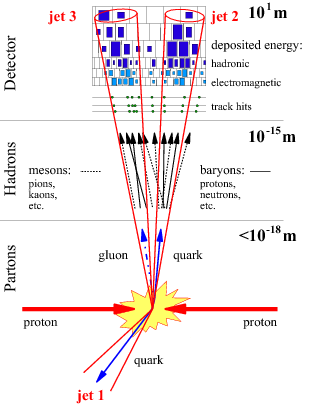
\includegraphics[width=0.4\linewidth]{Pics/cp4/41.png}
  	\caption{Illustration of jets at different scales. The jets can be characterized in three different stages, the so-called parton, hadron (particle) and detector level~\cite{Carli:2015qta}.}
   	\label{fig:41}
\end{figure}


\subsubsection{Jet reconstruction}
 For this analysis the jet reconstruction software FastJet 2.4.3~\cite{Cacciari:2011ma} is used to reconstruct jets formed at the electromagnetic (EM) scale from topological calorimeter cell clusters~\cite{Lampl:1099735}.  The anti-k$_T$ reconstruction algorithm~\cite{Cacciari:2008gp} is used with a radius parameter of $R$ = 0.4.
Calorimeter cells, where the deposited energy exceeds a certain noise threshold, are grouped to topological clusters. This noise threshold is obtained from measurements of the electronic noise of the calorimeter system and simulations of the pile-up noise~\cite{Aaboud:2017jcu}. 
 The clustering is performed by the anti-k$_T$ algorithm, which starts by calculating the distance of two distinguishable particles $i$ and $j$: 
\begin{equation}
d_{i,j} = min(k_{T,i}^{-2}, k_{T,i}^{-2})\frac{(\Delta R_{i,j})^2}{R^2}.
\end{equation}
$k_{T,i}$ denotes the transverse momentum of the particle $i$, while $\Delta R_{i,j}$ is the geometrical distance between the two particles in the detector coordinates (see~\cref{dinstance}).
The radius parameter $R$ determines  the size of the jet.
In addition to $d_{i,j}$, the distance to the beam pipe $d_{\rm i,beam}=k_{T,i}^{-2}$ for each single particle is calculated. Those two parameters are compared, for the shortest distance. If $d_{i,j}$ is smaller than $d_{\rm i,beam}$, the entities $i$ and $j$ are recombined. In the vice versa case, $i$ is referred to be a jet and removed. This procedure is repeated until all possible jet contributions are either absorbed into the jet candidate or removed.



\subsubsection{Jet calibration }

 The reconstructed jets are built from calorimeter clusters obtained at a certain energy scale, determined by the deposited energy. The jet energy scale (JES) is calibrated in several consecutive steps derived from a combination of MC-based simulation and in-situ methods. The calorimeter jets are obtained at the electromagnetic (EM) scale and corrected in their orientation. Therefore, the four-momenta of the jets are orientated to point towards the primary vertex of the hard interaction, which results in an improvement of the $\eta$ resolution.  In the next calibration step, pile-up effects are removed, by the subtraction via the area-based $p_T$ method~\cite{Cacciari:2007fd} and  residual corrections are applied to the  jets in data.  The  average momentum contamination from pile-up is subtracted from each jet momentum, depending on the jet area $A$. The average $p_T$ per event density in the $\eta-\phi$ plane is calculated and for each jet taken to be $p_T/A$, using ghost particles. The measurement of the number of ghost particles,  allows to determine the size of the  jet area $A$.~\cite{Aaboud:2017jcu}

 In order to reject jets originating from pile-up events,  additional cuts are applied. For jets with  $p_T <$ 60~GeV and within  0 $<\mid \eta \mid<$ 2.4,  a track-based technique is used, which rejects  jets from pile-up by the jet vertex tagger (JVT). Moreover, the effects of out-of-time pile-up, are taken into account via the application of  a residual correction, which is derived from comparisons to truth particle jets in simulated dijet events.~\cite{Aad:2015ina}


 The calorimeter clusters are calibrated using the EM-JES calibration scheme, where the jet four-momenta is adopted to the particle-energy scale by the absolute JES calibration. In addition, the energy scale of the reconstructed jets are corrected with the information from the calorimeter, the MS and track-based variables. Furthermore, corrections are applied with a residual in-situ calibration to correct jets in data using well-measured reference objects, e.g.  photons, $Z$-bosons and calibrated jets.~\cite{Aaboud:2017jcu}

 Finally, an overlap removal is applied, which prevents the double-counting of electrons as a jet. Therefore, the closest jet  to an electron, within a cone of $\Delta R $ < 0.2, is removed. Furthermore, electrons in a cone $\Delta R $ < 0.4 around a jet are rejected. The same is done for muons, if the jet can be associated to at least three tracks, otherwise the jet is removed.



\subsection{Tagging of $b$-Jets}
In the measurement of the top-quark mass, the identification of jets originating from $b$-quarks is particularly important, since  top quarks almost exclusively decay into $b$-quarks and a $W$-boson (see~\cref{decay1}). This can be done using the fact that the hadrons containing a $b$-quark have a significant  lifetime, which results in a relatively large propagation of those so-called $B$-hadrons, until the decay. The  large distances, which the particles travel in the detector allow to distinguish them from non-$B$-hadrons.   
The  jets  from $b$-quarks can thus be identified by the reconstruction of the $B$-hadron decay vertices, due to a noticeable shift of the  jet axis and a large impact parameter (see~\cref{fig:42}). These jets are referred in the following as $b$-jets, while jets associated with hadrons from lighter quarks, $u, d, s, c$ or gluons are called light jets.

On the one hand, $b-$tagging offers the huge advantage to improve the event selection by applying cuts on the number of tagged jets, thus reducing certain background contributions. On the other hand, it is a cornerstone for the kinematic reconstruction of the event, since it allows to distinguish the $b$-jets from the light jets of the $W$-boson decay. 

\begin{figure}[h]
	\centering
	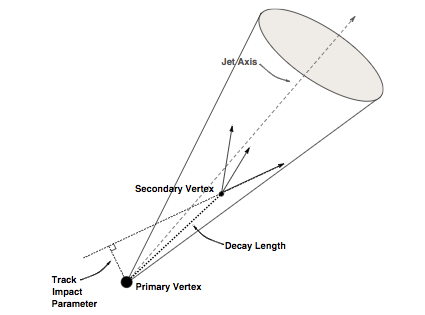
\includegraphics[width=0.5\linewidth]{Pics/btag.png}
	\caption{ Illustration of the $b$-jet reconstruction, with the characteristic decay length between the primary and secondary vertex ~\cite{ATLAS:2010rza}.} 
	\label{fig:42}
\end{figure}

The $b$-jet identification in this thesis is based on the MV2c10 method~\cite{ATL-PHYS-PUB-2016-012}, which combines the results of the three standard  $b$-tagging algorithms, which are taking the jet $p_T$ and the $\eta$ region into account.

 The first algorithm is the IP3D, which is a lifetime-based tagging method~\cite{ATL-PHYS-PUB-2016-012}. In addition, the inclusive multi-vertex finding algorithm JetFitter~\cite{Piacquadio:2008zza} is applied, followed by a secondary vertex reconstruction with the SV algorithm~\cite{ATLAS-CONF-2011-102}.

 The output of the three basic  tagging algorithms are combined with a Boosted Decision Tree (BDT)~\cite{ATL-PHYS-PUB-2016-012}. 
The information of the three algorithms is 
 used to calculate a discrimination weight $w$ within the multivariate analysis, which represents  the probability of a certain jet  to contain a $B$-hadron.  While for $b$-jets, this weight is close to unity, light jets can be associated to small values of $w$.


 
A $b$-tagging working point (WP) is chosen by constraining $w$ via specific cuts, to determine the efficiency of the tagging algorithm, i.e. the probability that a jet is correctly identified as $b$-jet. 
 Furthermore, a rejection factor is taken into account.  Here,the chosen working point, belongs to an average $b$-tagging efficiency of 77~\%, obtained in simulated $t\bar{t}$ events. For jets referred to  $c$-hadrons, the rejection factor is 6.2, while for lighter flavoured  hadrons it is 134. 
 


\subsection{Missing transverse  energy}\label{ET}

The transfers energy ($E_T$)  is determined with the cell structure of the calorimeter system.  For a physical object, the transverse energy can be calculated with:
\begin{equation}
E_T = E sin(\theta).
\end{equation}
$E$ is the measured energy, which belongs to the corresponding calorimeter cells of the jet. The polar angle ($\Theta$)  provides the information  about the  direction of the jet with respect to the beam pipe. 

 

$E^{\rm miss}_T$ is defined as the negative vector sum of the transverse momentum $p_T$ of all selected physical objects. Furthermore, an additional so-called soft term is taken into account, considering disturbances like the false reconstruction of tracks.
A certain amount of missing transverse energy $E^{miss}_T$ ~\cite{ATL-PHYS-PUB-2015-027} can arise due to weakly interacting particles in the final state, e.g. the neutrino in the $t\bar{t}\rightarrow$ lepton + jets channel or from energy leakage effects in the detector.

 For the determination of $E^{miss}_T$, Monte Carlo simulation is compared to data of the year 2015, with a track-based soft term (TST) ~\cite{ATL-PHYS-PUB-2015-027}. The soft-term is reconstructed from Inner Detector tracks, which are associated with the primary vertex of the selected physical objects and provide  information about the non-selected contribution.  
The missing transverse energy is built per event.


 



\section{Data and Monte Carlo samples}\label{DATA}

This analysis is based on the data taken in 2016 with the ATLAS detector, obtained from  $pp$ collisions at a center-of-mass energy of $\sqrt{s}$= 13~TeV, with a corresponding luminosity of 33~fb$^{-1}$. For several purposes of this analysis, e.g. the simulation of the different signal and background contributions or the estimation of interactions with the detector material, Monte Carlo generators (MC) are used. 



The matrix elements (ME) of the signal $t\bar{t}$ samples are simulated at next-to-leading order (NLO), using the \textsc{Powheg-Box v2} generator%(r3026)
~\cite{Nason:2004rx,Frixione:2007vw,Alioli:2010xd}, with the \textsc{NNPDF 3.0} parton distribution function (PDF) ~\cite{Ball:2014uwa}. The parton shower is modelled in leading-order (LO) with \textsc{Pythia 6}~\cite{Sjostrand:2006za} in perturbative QCD, with the~\textsc{NNPDF 2.3} PDF~\cite{Ball:2012cx}  and the \textsc{Perugia 2012} tune~\cite{Skands:2010ak}.
The hadronization and  underlying events are also modelled  with the \textsc{Pythia 6} program. In addition, the nominal $t\bar{t}$ sample ($m_{\text{top} }$= 172.5~GeV)  is also produced with \textsc{Pythia 8}~\cite{Sjostrand:2007gs} , the same PDF sets and the A14 tune~\cite{ATL-PHYS-PUB-2014-021}.
The top-quark mass is assumed to be 172.5~GeV and the damping parameter $h_{\rm damp}$, which regulates the $p_T$ emissions beyond the Born parton shower (PS) configuration, is chosen to be 1.5~m$_{\rm top}$ for  \textsc{Powheg + Pythia 8} and 1.0~m$_{\rm top}$ for  \textsc{Powheg + Pythia 6}.


For the NLO matrix element of the single top events, the \textsc{Powheg-Box v1} generator with the \textsc{CT10} PDF~\cite{Lai:2010vv} is used. The parton shower is also simulated in LO with the  \textsc{Pythia 6} program, using the \textsc{CTEQ6L1}~\cite{Pumplin:2002vw} PDF and the \textsc{Perugia 2012C} tune.  While the top-quark mass is assumed to be 172.5~GeV. There is no  $h_{\rm damp}$ for single top quarks.


  $W$- and $Z$-boson events with jets are modelled using the  \textsc{Sherpa 2.2.1} MC generator~\cite{Gleisberg:2008ta,Schumann:2007mg,Hoeche:2012yf}, which provides the matrix elements in  NLO.  The corresponding PDF is  \textsc{NNPDF 3.0}. \textsc{Sherpa} is also used for the simulation the ME and the PS of diboson processes ($WW$, $WZ$ and $ZZ$) in NLO, interfaced with the \textsc{CT10} PDF set. $t\bar{t}V$ processes are events with a top-quark pair and a $W$- or a $Z$-boson. The ME is calculated in NLO with the MG5\_aMC@NLO generator~\cite{Alwall:2014hca}, with \textsc{NNPDF 3.0} and  \textsc{Pythia 8} with~\textsc{NNPDF 2.3} and the \textsc{A14} tune.

 The impact of multi-$pp$ collisions, is simulated for all samples by soft QCD processes with the \textsc{Pythia 8}  program. The applied parameter set is provided from the \textsc{A2} tune~\cite{ATL-PHYS-PUB-2012-003}, while the \textsc{MSTW2008LO} PDF ~\cite{Martin:2009iq} is taken.

 For mass hypotheses testing, $t\bar{t}$ samples are derived for different mass points, with $m_{\text{top}}$ = 170.0, 171.5, 172.5, 173.5 and 175. The signal MC samples are normalised for $m_{\text{top}}$ = 172.5~GeV to a cross-section of 832 $\pm$ 46~pb, calculated with the \textsc{Top++ 2.0} framework~\cite{Czakon:2011xx} in next-to-next-to-leading-order QCD and with 
the resummation of next-to-next-to-leading logarithmic soft gluon terms~\cite{Cacciari:2011hy,Beneke:2011mq,Baernreuther:2012ws,Czakon:2012zr,Czakon:2013goa}.  For the normalization of the background samples, the corresponding  theoretical cross-sections are calculated in at least NLO  QCD~\cite{Catani:2009sm,Kidonakis:2010tc,Kidonakis:2010ux,Kidonakis:2011wy,Campbell:1999ah,Campbell:2011bn,Alwall:2014hca,deFlorian:2016spz,ATL-PHYS-PUB-2016-003}. 
 



 In order to consider the  interactions with the detector material, each simulated sample has to undergo the ATLAS detector and trigger simulation~\cite{Aad:2010ah}. Therefore, \textsc{Geant 4}~\cite{Agostinelli:2002hh}  is used to simulated the interactions with the detector components.  In addition, for the evaluation of systematic uncertainties, signal MC samples are produced with the much faster \textbf{Atlfast 2.0}~\cite{Richter-Was:683751} simulation. This method leaves the simulation of the inner detector system unchanged, while using a faster approximation for the energy deposition in the calorimeter system.

 In addition to the samples produced for the data/MC comparison further samples are needed for the evaluation of the systematic uncertainties. More details can be found in~\cref{sec:Uns}. 



\section{Event preselection and background contributions}\label{selection}
 One of the most difficult tasks at modern hadron collider experiments is the handling of the large amount of data and the selection of the interesting physical processes. Therefore, analysis dependent quality criteria are applied, taking the characteristic event topology of the  $t\bar{t}\rightarrow$ lepton + jets into account. In addition, the chosen selection cuts try to minimize the background contamination of the signal region. 
 
 In the following, the different background contributions for the lepton + jets channel will be discussed, before the applied event triggers and selection cuts are presented together with the control distributions of the observables.
 
 
 \subsection{Single top background}
 
 In the phase space of the $t\bar{t} \rightarrow$lepton + jets decay, several background processes contribute to the measurement.  Those background events are able to pass certain selection criteria and can be misidentified as signal events.
 
 Single-top events are a major background process, due to the presence of the top-quarks. They can lead to a simultaneous event structure and  event kinematic as of the lepton + jets  decay channel. However, there is a noticeable mass dependence of single-top events, which is the reason why it has been added to the signal region in the previous analyses~\cite{ATLAS-CONF-2017-071, Aad:2015nba}. Nevertheless, in terms of this thesis, single top events are referred to as background, due to missing MC samples for the different mass points\footnote{Only the nominal sample for 172.5~GeV is available for single-top production.}. 
 
 \subsection{Diboson background}
 The top-quark mass measurement is also affected by final states with two $W$-bosons, two $Z$-bosons or the combination of a $W$- and a $Z$-boson.  If one of the two bosons decays leptonically, while the other one decays into hadrons, this can lead to the mis-identification with the detector signature of the lepton + jets final state.  
 

 \subsection{$W$ + jets background}
The main background source  are $W$ + jets events. This event type arises from $W$-boson production together with strongly interacting particles (quarks and gluons), which end up as additional jets. Particular events, where the $W$-boson decays leptonically, can lead to detector signatures, which can easily be mis-identified with $t\bar{t} \rightarrow$ lepton + jets events.



 \subsection{$Z$ + jets background} 
In addition to the $W$ + jets background, there are also events with a leptonically decaying $Z$-boson, which, together with hadronically decaying particles, have a similar detector signature as the  $t\bar{t} \rightarrow$ lepton + jets final state. As shown in the following, the $Z$ + jets background is about one magnitude smaller than the $W$ + jets background and can be easily suppressed by requesting exactly one charged lepton and $b$-jets.



\subsection{Multijet/non-prompt lepton background}
QCD-multijet events are final states which do not contain any primary leptons. They only arise from hard-scattering processes of strongly interacting particles (quarks and gluons). However, some hadronic jets can be misidentified as electrons, due to the energy deposition in the Electromagnetic Calorimeter. One refers to these jets as fake-lepton background. Furthermore, weak hadron decays inside of an hadronic jet, lead to the identification of further leptons, which might be able to pass the isolation criteria (non-prompt leptons).
The consideration of the non-prompt/fake lepton background is very important, due to the fact that this contributions can be mis-identified with the charged isolated leptons arising from the $W$-boson decay of the $t\bar{t}$ final state.

The background has not been estimated yet and will not be included in this thesis.
 
 

 \subsection{Event triggering}
 In context of this measurement, events containing single leptons (electrons and muons) are selected using different single lepton triggers.
 For each case of the $t\bar{t} \rightarrow$ lepton + jets decay, several  trigger options for the single leptons are available, which do not take any further hadron information into account. The used trigger setup is given in~\cref{tab:trigr2}.
 

 \begin{center}
 	\captionof{table}{Trigger setup for electrons and muons. }\label{tab:trigr2}
 	
 	
 	
 	\vspace{0.3cm}	
 	
 	
 	\begin{tabular}{>{}m{7.0cm}>{}m{3.0cm}>{}m{3.0cm}} \toprule
 			Trigger&  lepton&$p_T$ cut /[GeV]\\
 			\midrule
 		
 		HLT\_e26\_lhtight\_nod0\_ivarloose& electron&  26\\
 		HLT\_e60\_lhmedium\_nod0  & electron&  60 \\
 		HLT\_e140\_lhloose\_nod0& electron &140\\
		HLT\_mu26\_ivarmedium & muon & 26\\
		HLT\_mu50 & muon & 50\\
 	

 		
 		\bottomrule
 	\end{tabular}
 	
 \end{center}
 
 
 
 
 
 
 
 
\subsection{Preselection criteria} 
In order to obtain the $t\bar{t} \rightarrow$ lepton + jets events and perform an efficient separation from background, one uses the fact that each of the interesting events can be identified by its characteristic decay topology, with  two $b$-jets and at least two light jets. Furthermore, the detector signature contains one charged isolated lepton and the corresponding neutrino, which can only be registered by considering the missing transverse energy $E^{miss}_T$. Preselection cuts are applied to obtain events with these criteria using a similar selection as for the previous analyses for 7~TeV~\cite{Aad:2015nba} and 8~TeV~\cite{ATLAS-CONF-2017-071}:




\begin{itemize}
	\item  At least one good primary vertex has to be obtained for selected events\footnote{The primary vertex is the one  with the highest   $\sum p_T^2$, where  $p_T$ denotes the transverse momentum and the sum runs over all associated  tracks.}.
	\item In addition the single-electron or single-muon  trigger has to have fired.
	\item The triggered leptons are further required to have a transverse energy of $E_T > $ 27~GeV for electrons, while for muons, the transverse momentum $p_T$  must exceed 27~GeV. 
	\item For the electron + jets channel, additional cuts are applied:  $E_T^{\rm miss}$ > 30~GeV,  $m_T^W$ > 30~GeV\footnote{The transverse $W$ mass is defined as: $m_T^W$ =$\sqrt{2p_T^lE_T^{\rm miss}(1-cos\phi(l,E^{\rm miss}_T))}$, where $l$ denotes the properties related to the charged lepton.} and $E_T^{miss} + m_T^{W} > 60$~GeV.
	\item Events with a muon are required to have a missing transverse energy of at least
	20~GeV  and to fulfil the relation: $E_T^{\rm miss} + m_T^{W} > 60$~GeV.
	\item Furthermore, events are only selected if they contain at least four jets, with a $p_T$ above 25~GeV in the central region of the detector ($\mid \eta \mid $ < 2.5).
	\item At least one of the jets  has to be tagged as a $b$-jet. 
\end{itemize}

 In addition to the preselection cuts there are analysis specific cuts on some global quantities in analogy to~\cite{ATLAS-CONF-2017-071}. These quantities, e.g. the constructed top-quark mass, belong to result  from the event reconstruction and will be discussed in detail in~\cref{ch5}, together with the results of the preselection.





















\clearpage
